
\section{Voltage regulator for bracelet}
The voltage regulator is needed to regulate voltage from the battery to GPS module and RF module in the bracelet.
Firstly, the prototype was done in the lab. When the test was done and succesfull, it was implememnted in the PCB for the bracelet.\\
The voltage regulator was created using LM-317T, because it is an adjustable voltage regulator and gives possibility to 
change the output voltage if the potentiometer is used in the circuit or with changing one of the resistors only.  

To find the right resistors there must be used an equation: 
\begin{equation}\label{Eq: LM317T}
    V_{out}=1.25*(1+\frac{R_{2}}{R_{1}})
\end{equation}
$R_1$ - set resistor, was chosen to be 100 Ω \\
$R_2$ - adjustable resistor \\
$V_{out}$ = 3.3 V, later measured to be 3.27 V \\
$V_{battery}$=7.51 V (measured)\\
From eq. (\ref{Eq: LM317T}): $R_2$ = 160 Ω \\

To check if the circuit works as needed, load resistor is added. The load resistor is expceted to act as two modules that would 
be attached to voltage regulator output. \\
To find the $R_{load}$, maximum currents needed by modules are found in their datasheets and then add 20\% for assuring.\\
\[GPS:\; I_{max} = 100mA + 20\% = 120mA \]
\[RF:\; I_{max} = 13.5mA + 20\% = 16.2mA \]
Adding them:
\[120mA+16.2mA = 136mA\]
\[R_{L}=\frac{V}{I_{max}}=\frac{3.27V}{136mA} = 24.0444 \Omega\]
The resistor available in the lab was 24$\Omega$ and measured to be 24.2$\Omega$.\\
\begin{figure}[H]
    \centering
    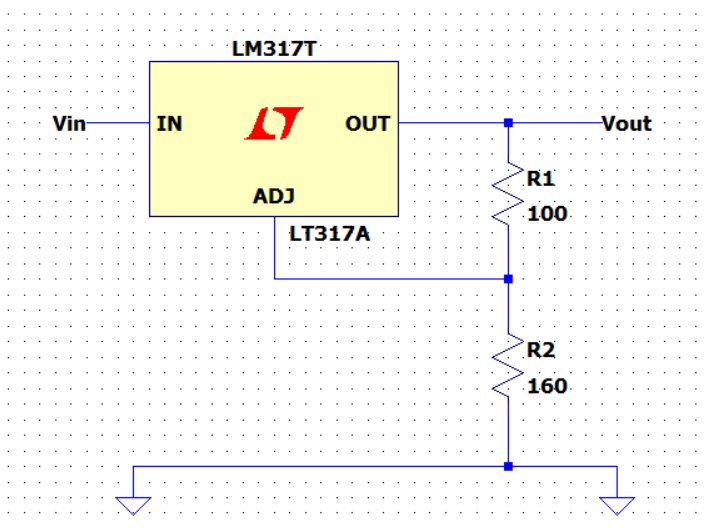
\includegraphics[width=0.7\textwidth]{voltagereg_circuit.png}
    \caption{Voltage Regulator Testing Circuit}
    \label{Figure: Voltage Regulator Testing Circuit}
\end{figure}
\begin{figure}[H]
    \centering
    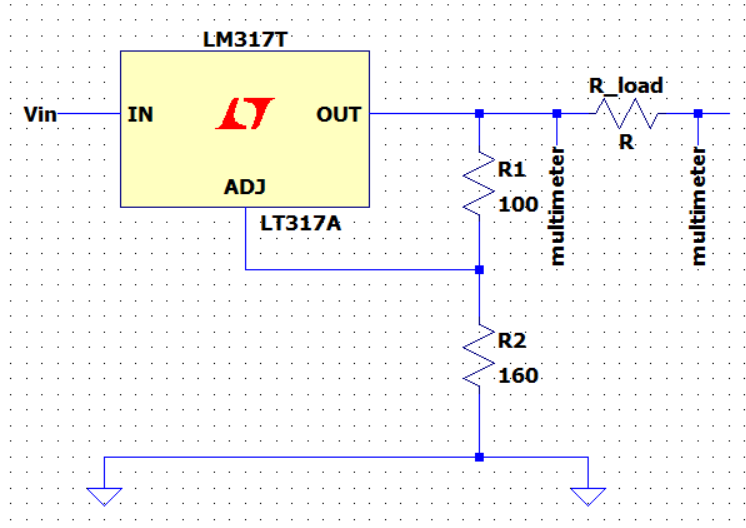
\includegraphics[width=0.7\textwidth]{testin_voltagereg_circuit.png}
    \caption{Voltage Regulator Circuit}
    \label{Figure: Voltage Regulator Circuit}
\end{figure}
\begin{figure}[H]
    \centering
    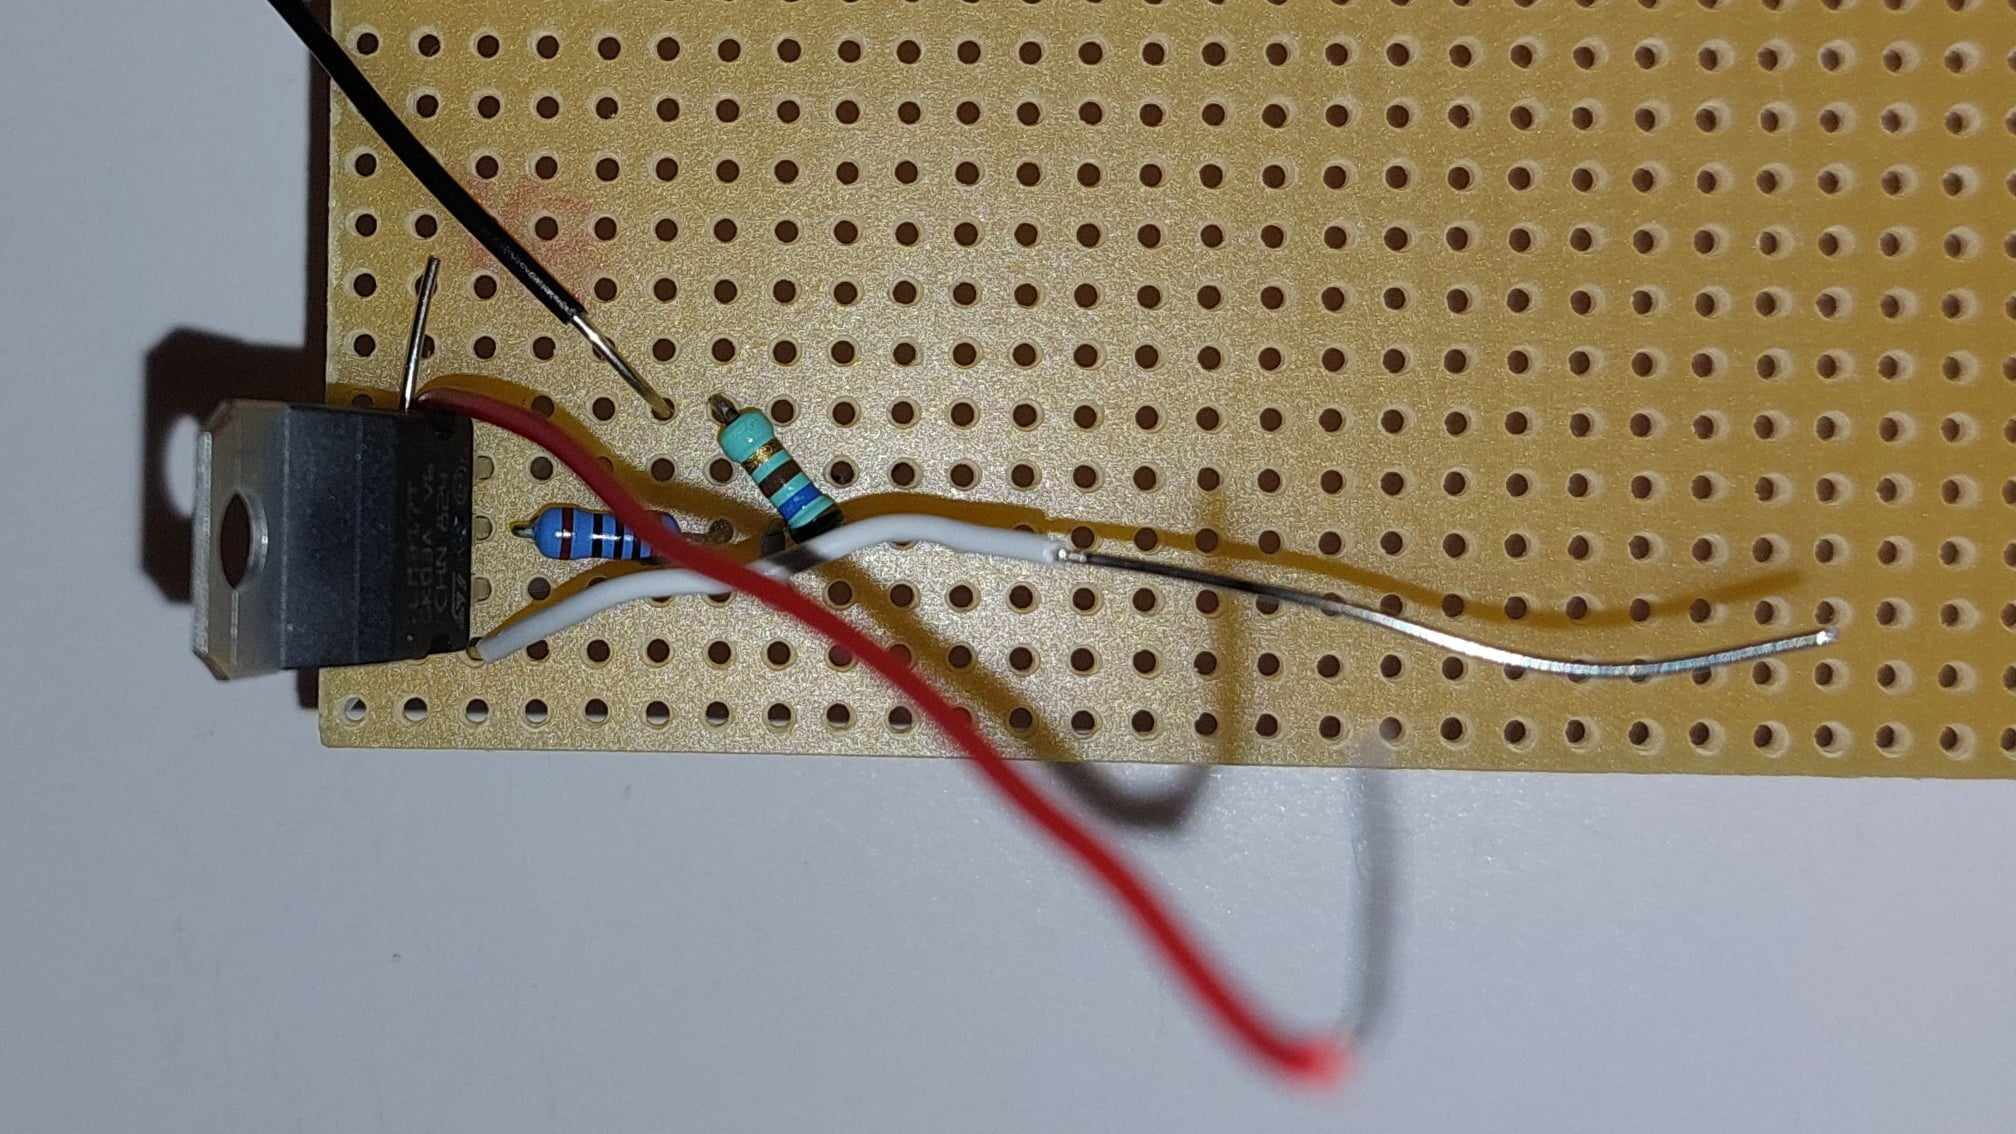
\includegraphics[width=0.7\textwidth]{voltagereg.jpg}
    \caption{Voltage Regulator}
    \label{Figure: Voltage Regulator}
\end{figure}

After soldering the components, there was a short cicuit. However, with use of multimeter it was easily found and repaired. 
The voltage output was as expected and needed by the modules.